% Use only LaTeX2e, calling the article.cls class and 12-point type.

\documentclass[12pt]{article}

% Users of the {thebibliography} environment or BibTeX should use the
% scicite.sty package, downloadable from *Science* at
% www.sciencemag.org/about/authors/prep/TeX_help/ .
% This package should properly format in-text
% reference calls and reference-list numbers.

\usepackage{scicite}

% Use times if you have the font installed; otherwise, comment out the
% following line.

\usepackage{times}

\usepackage{enumitem}
\usepackage{float}
\usepackage{graphicx}
\usepackage{subcaption}
\usepackage[table,xcdraw]{xcolor}

% The preamble here sets up a lot of new/revised commands and
% environments.  It's annoying, but please do *not* try to strip these
% out into a separate .sty file (which could lead to the loss of some
% information when we convert the file to other formats).  Instead, keep
% them in the preamble of your main LaTeX source file.


% The following parameters seem to provide a reasonable page setup.

\topmargin 0.0cm
\oddsidemargin 0.2cm
\textwidth 16cm 
\textheight 21cm
\footskip 1.0cm


%The next command sets up an environment for the abstract to your paper.

\newenvironment{sciabstract}{%
\begin{quote} \bf}
{\end{quote}}


% If your reference list includes text notes as well as references,
% include the following line; otherwise, comment it out.

\renewcommand\refname{References and Notes}

% The following lines set up an environment for the last note in the
% reference list, which commonly includes acknowledgments of funding,
% help, etc.  It's intended for users of BibTeX or the {thebibliography}
% environment.  Users who are hand-coding their references at the end
% using a list environment such as {enumerate} can simply add another
% item at the end, and it will be numbered automatically.

\newcounter{lastnote}
\newenvironment{scilastnote}{%
\setcounter{lastnote}{\value{enumiv}}%
\addtocounter{lastnote}{+1}%
\begin{list}%
{\arabic{lastnote}.}
{\setlength{\leftmargin}{.22in}}
{\setlength{\labelsep}{.5em}}}
{\end{list}}


% Include your paper's title here

\title{Reduction of Convolutional Layers in Deep Networks} 


% Place the author information here.  Please hand-code the contact
% information and notecalls; do *not* use \footnote commands.  Let the
% author contact information appear immediately below the author names
% as shown.  We would also prefer that you don't change the type-size
% settings shown here.

\author
{Vincent Martineau,$^{1\ast}$\\
\\
\normalsize{$^{1}$Department of Computer Science and Software Engineering, Université Laval, Quebec, Canada}\\
\\
\normalsize{$^\ast$E-mail:  vincent.martineau.1@ulaval.ca.}
}

% Include the date command, but leave its argument blank.

\date{}



%%%%%%%%%%%%%%%%% END OF PREAMBLE %%%%%%%%%%%%%%%%



\begin{document} 

% Double-space the manuscript.

\baselineskip24pt

% Make the title.

\maketitle 



% Place your abstract within the special {sciabstract} environment.

\begin{sciabstract}
  
  There has been research explaining how to reduce convolutional layers in neural networks. However in the proposed articles the models used are usually AlexNet and VGG. When tried on more complex networks such as ResNet, DenseNet and SqueezeNet the proposed solutions do not work. The goal here is to explore the limits of this approach and to propose a solution in order to generalize to more complex and deep networks than those in Molchanov's original article. Experiments will be done on the model transfer between ImageNet to Cifar10 and we will see the gains that can be.
\end{sciabstract}



% In setting up this template for *Science* papers, we've used both
% the \section* command and the \paragraph* command for topical
% divisions.  Which you use will of course depend on the type of paper
% you're writing.  Review Articles tend to have displayed headings, for
% which \section* is more appropriate; Research Articles, when they have
% formal topical divisions at all, tend to signal them with bold text
% that runs into the paragraph, for which \paragraph* is the right
% choice.  Either way, use the asterisk (*) modifier, as shown, to
% suppress numbering.

\section*{Introduction}

CNN networks have been with us for a very long time \cite{lecunn1}. These networks are widely used in image processing in a wide variety of fields. They are very used in the classification or location of objects. Whether with surveillance systems, autonomous cars or smart devices, this type of network is now part of our daily work \cite{daily}.

These networks have shown that they can achieve results beyond human capabilities \cite{beathuman}. In many cases, these models are made available to the general public and can be adapted to simpler problems to get very good results \cite{transfer}.

\subsection{Description of the problems}
In order to use these safe networks of small devices \cite{han1} techniques have been evaluated in the past. More recently, an article proposes to make the reduction of convolution filters \cite{molchanov}. However the article focuses mainly on AlexNet and VGG networks and does not work on the more complex networks present in PyTorch \cite{pytorchmodel}.

The purpose of this article will be to evaluate the work needed to push this logic to more complex networks such as ResNet, DenseNet and SqueezeNet.

\section*{Method}
\setcounter{subsection}{0}
The method used is a variant of the method proposed in the article Pruning Convolutional Neural networks for Resource efficient inference \cite{molchanov}. The purpose of the changes is to extend the capabilities of our model to much more complex networks such as ResNet, DenseNet and SqueezeNet.

Here is a list of the steps to follow to get an interesting result:
\begin{enumerate}[noitemsep, noitemsep]
	\item Apply fine tuning on a pre-trained network.
	\item Extract the execution graph from our model.
	\item From our execution graph, exclude convolutional layers that we do not want to affect.
	\item Reduce the filters according to the reduction criterion.
	\item Apply fine tuning to restore the network.
	\item Repeat the reduction until the network is the size you want.
\end{enumerate}

In this procedure the selection criterion is very important to have good results. For this experiment, we used the Taylor Expansions which proved their effectiveness in the article and the average activations.

In order to be able to run on more complex models, we chose not to explore other selection criteria, but to focus on the algorithm needed to support more complex models.

\subsection{The layers to ignore }
In the proposed solution, it is important not to apply filter reduction just before a flow addition as seen in several complex models. Figure 1 represents this situation. The problem in this case is that it is necessary to apply an equivalent reduction on all incoming branches. It is possible that there is a selection criterion to include these layers in the future.

\begin{figure}[H]
	\centering
	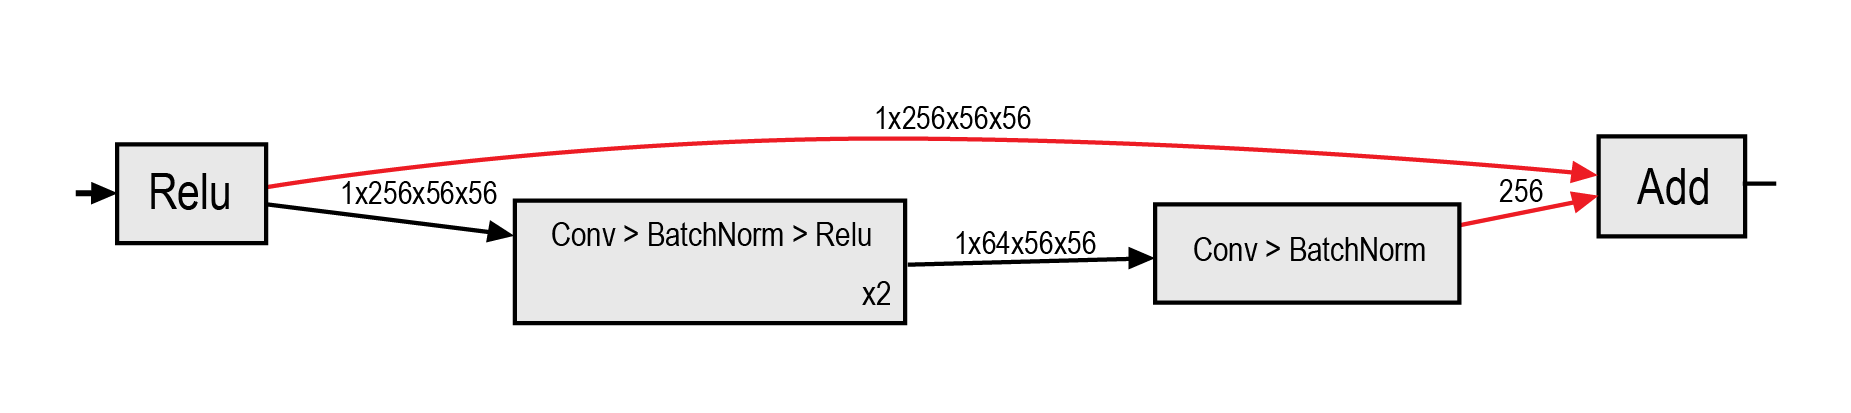
\includegraphics{fig/residual_add}
	\caption{In the following figure it is impossible to reduce the second convolution layer for the bottom branch since it would also be necessary to modify the layer preceding this ResNet block so that the residual connection has the right size.}
	\label{fig:residualadd}
\end{figure}

Another potential problem occurs when a layer is reused. In this case it is necessary that the input of our layer is compatible with the exit of the layer which we treat. However, we must assign the previous layers so that the dimensions are also consistent.
\newpage
Note that it is possible that there is a reliable algorithm that can handle these cases, but this article does not explore these options.

Finally, it is crucial not to affect a layer if it directly influences the number of network outputs. Such a practice would directly affect the performance and training of the model. There could be a lag between classes during classification and the loss function could become invalid.

\subsection{Practices to avoid}

When a model is created it is important to avoid hardcoded value in the inference function. For example, in the AlexNet model, there is the code on the left side of Figure 2 that prevents us from reducing the last convolution layer before the fully connected layer. By performing the modification shown in Figure 2, it is now possible to reduce the convolution layer before the fully connected layer.
\begin{figure}[H]
	\centering
	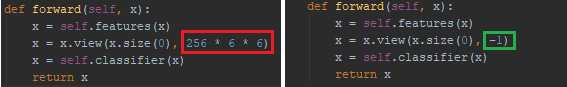
\includegraphics{fig/mistake}
	\caption{Note in the left-hand section that the original code assumes a fixed size for the last convolution layer. In addition to limiting the model to a certain input image size, the last convolution layer can not be reduced. The proposed solution requires the modification in the right section of the image that allows a variable size of the last convolution layer.}
	\label{fig:mistake}
\end{figure}


\subsection{Propagation of the effect}
When we remove a convolution filter from a layer, several precautions must be taken to ensure the stability of the system. For example, we must adjust the weights, the number of skewings in the layer and adjust the gradients when they are contained in the layer itself. Which is the case of PyTorch.
\newpage
Subsequently, the following layers must be adjusted according to their type.
\begin{itemize}[noitemsep, noitemsep, label={}]
	\item For the following \textbf{convolutions} layers. It is necessary to adjust the number of layers in inputs to match the convolutional layer we are dealing with. We must also adjust the weight of this layer.
	\item For \textbf{Batchnorm} layers, we must adjust the bias when used and we reset the variables used at runtime. In PyTorch, we talk about running means and running vars.
	\item Finally, we need to adjust \textbf{fully connected} layers. In the case of these layers, we adjust the weights and apply the \textit{weight inference rule} \cite{weightinference} to simulate weight removal by \textit{dropout}.
\end{itemize}

The other layers seem to support the reduction of convolutional layers. It should be noted that we have only tried the models proposed in PyTorch and that other work might be needed for more complex layers.

\section*{Résultats}
First, we evaluate the effect of reducing convolution filters on the AlexNet model. Figure 3 shows the effects of the reduction. The first result we can notice is that a succession of too much pronounced reduction significantly reduces the pre-workout effect.
\begin{figure}[H]
	\centering
	\begin{subfigure}[b]{0.33\textwidth}            
		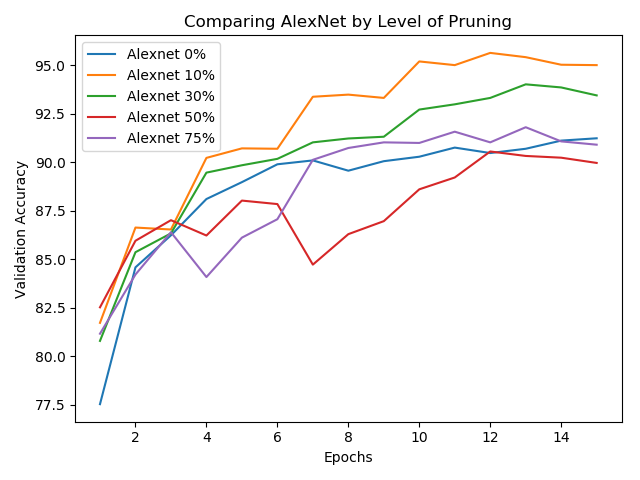
\includegraphics[width=\textwidth]{fig/prune_ratio_rough}
		\label{fig:pruneratiorough}
	\end{subfigure}%
	%add desired spacing between images, e. g. ~, \quad, \qquad etc.
	%(or a blank line to force the subfigure onto a new line)
	\begin{subfigure}[b]{0.33\textwidth}
		\centering
		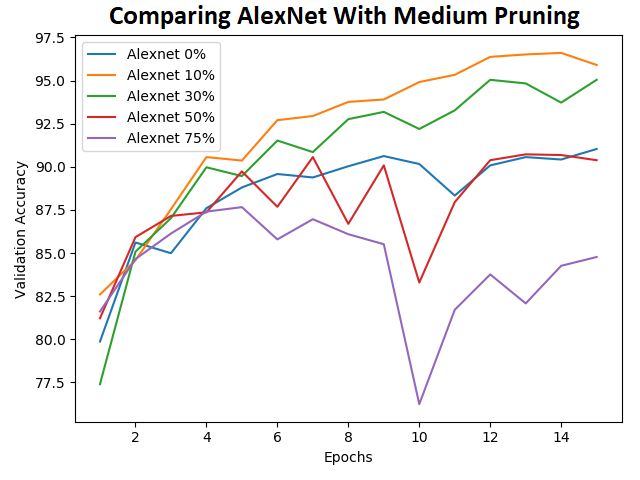
\includegraphics[width=\textwidth]{fig/prune_ratio_medium}
		\label{fig:pruneratioslow}
	\end{subfigure}
	\begin{subfigure}[b]{0.33\textwidth}
		\centering
		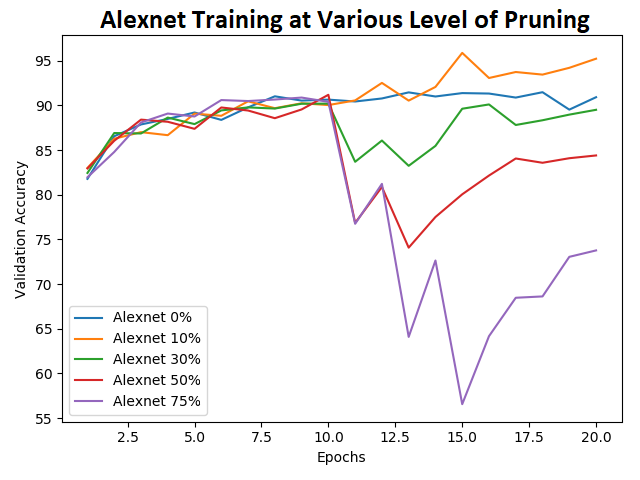
\includegraphics[width=\textwidth]{fig/prune_ratio_slow}
		\label{fig:pruneratioslow}
	\end{subfigure}
	\caption{In the figure on the left, there is a significant reduction of the weights at each iteration over two iterations (epoch 4 and 7). The figure of the center represents a reduction on 5 iterations with 2 steps of leveling. In the figure on the right, we see a more gradual reduction made over 10 iterations.}
\end{figure}

\begin{table}[H]
	\centering
	\caption {\textbf{Comparison of results after model reduction}}
	\begin{tabular}{clllll}
		\textbf{}                & \multicolumn{1}{c}{\textbf{0\%}} & \multicolumn{1}{c}{\textbf{10\%}} & \multicolumn{1}{c}{\textbf{30\%}} & \multicolumn{1}{c}{\textbf{50\%}} & \multicolumn{1}{c}{\textbf{75\%}} \\
		\textbf{Fast Pruning}    & 91.02                            & 88.94                             & 89.94                             & 88.01                             & 88.79                             \\
		\textbf{Average Pruning} &                                  &                                   &                                   &                                   &                                   \\
		\textbf{Slow Pruning}    & 90.74                            & 90.14                             & 89.43                             & 87.84                             & 81.02                            
	\end{tabular}
\end{table}

Figure 3 also shows an important aspect. It shows that the way to reduce weights is important. Reducing the weight too fast will cause more noise in the training. However, the number of training epochs performed after the last reduction seems essential to obtain good results. In contrast, we notice that a gradual reduction over a longer period brings more stability to the model for a certain time, but that the number of iterations of reduction eventually reduces the final performance of the model. An approach between the two gets good stability in the model and the final results are more consistent.

Then we compare the difference in efficiency between the models. This difference is visible in Figure 4 which compares the shallow models in the left section and the deep Pytorch models in the right graph. In any case, we note that even with a reduction of 30\% that can be cut, it is possible to significantly reduce the network and maintain a level of performance.

\begin{figure}[H]
	\centering
	\begin{subfigure}[b]{0.5\textwidth}            
		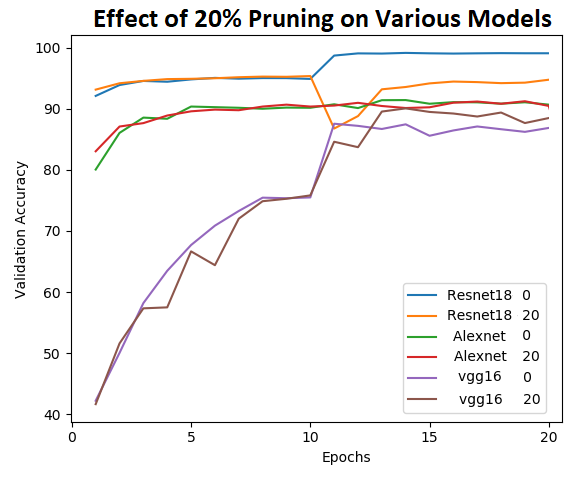
\includegraphics[width=\textwidth]{fig/various_models_shallow}
		\label{fig:SRl}
	\end{subfigure}%
	%add desired spacing between images, e. g. ~, \quad, \qquad etc.
	%(or a blank line to force the subfigure onto a new line)
	\begin{subfigure}[b]{0.5\textwidth}
		\centering
		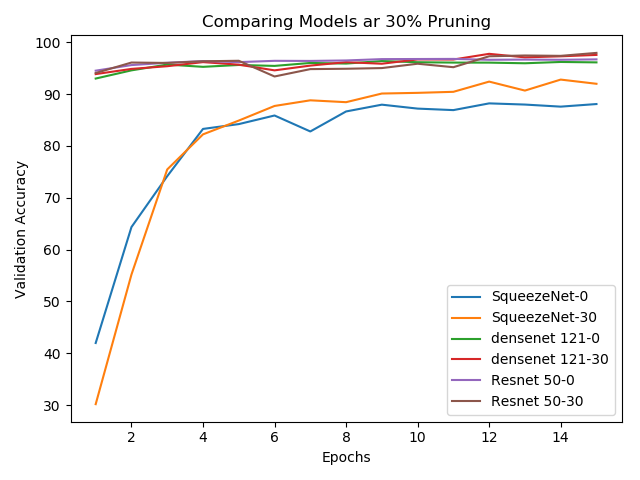
\includegraphics[width=\textwidth]{fig/various_models_deep}
		\label{fig:D-Imager}
	\end{subfigure}
	\caption{In the image on the left we can see the effect of the reduction on shallow models. In the image on the right we see the effect of the reduction on the deep networks of PyTorch.}
\end{figure}
The strategy used for the reduction is to make a gradual reduction. That is, cut 5 \% filters that can be reduced and repeat for 6 iterations. It can be seen that this strategy gives better results on all models at the validation level. However, we note that the final scores are slightly lower.
\begin{table}[H]
	\caption {\textbf{Comparison of the reduction according to the model}}
	\begin{tabular}{cccccccccc}
		\multicolumn{1}{l}{\textbf{}}           & \multicolumn{3}{c}{\textbf{VGG}}                                                                            & \multicolumn{3}{c}{\textbf{AlexNet}}                                                                        & \multicolumn{3}{c}{\textbf{ResNet18}}                                                                      \\
		\multicolumn{1}{l}{}                    & 0\%                       & 30\%                      & Diff                                                & 0\%                       & 30\%                      & Diff                                                & 0\%                       & 30\%                      & Diff                                               \\ \cline{2-10} 
		\multicolumn{1}{c|}{\textbf{FLOPs (G)}}  & \multicolumn{1}{l}{17.31} & \multicolumn{1}{l}{10.55} & \multicolumn{1}{l|}{{\color[HTML]{009901} -39.1\%}} & \multicolumn{1}{l}{0.815} & \multicolumn{1}{l}{0.500} & \multicolumn{1}{l|}{{\color[HTML]{009901} -38.7\%}} & \multicolumn{1}{l}{1.83}  & \multicolumn{1}{l}{1.40}  & \multicolumn{1}{l}{{\color[HTML]{009901} -23.5\%}} \\
		\multicolumn{1}{c|}{\textbf{Params (M)}} & \multicolumn{1}{l}{138.3} & \multicolumn{1}{l}{80.5}  & \multicolumn{1}{l|}{{\color[HTML]{009901} -42.8\%}} & \multicolumn{1}{l}{57.0}  & \multicolumn{1}{l}{47.9}  & \multicolumn{1}{l|}{{\color[HTML]{009901} -16.0\%}} & \multicolumn{1}{l}{11.18} & \multicolumn{1}{l}{7.53}  & \multicolumn{1}{l}{{\color[HTML]{009901} -32.6\%}} \\
		\multicolumn{1}{l|}{\textbf{Score (\%)}} & \multicolumn{1}{l}{91.92} & \multicolumn{1}{l}{92.03} & \multicolumn{1}{l|}{{\color[HTML]{009901} 0.11}}    & \multicolumn{1}{l}{90.98} & \multicolumn{1}{l}{88.57} & \multicolumn{1}{l|}{{\color[HTML]{9A0000} -2.41}}   & \multicolumn{1}{l}{94.8}  & \multicolumn{1}{l}{93.11} & \multicolumn{1}{l}{{\color[HTML]{9A0000} -1.69}}   \\ \hline
		\multicolumn{1}{l}{}                    & \multicolumn{1}{l}{}      & \multicolumn{1}{l}{}      & \multicolumn{1}{l}{}                                & \multicolumn{1}{l}{}      & \multicolumn{1}{l}{}      & \multicolumn{1}{l}{}                                & \multicolumn{1}{l}{}      & \multicolumn{1}{l}{}      & \multicolumn{1}{l}{}                               \\
		& \multicolumn{3}{c}{\textbf{SqueezeNet}}                                                                     & \multicolumn{3}{c}{\textbf{DenseNet121}}                                                                    & \multicolumn{3}{c}{\textbf{ResNet50}}                                                                      \\
		& 0\%                       & 30\%                      & Diff                                                & 0\%                       & 30\%                      & Diff                                                & 0\%                       & 30\%                      & Diff                                               \\ \cline{2-10} 
		\multicolumn{1}{c|}{\textbf{FLOPs (G)}}  & 0.516                     & 0.511                     & \multicolumn{1}{c|}{{\color[HTML]{009901} -0.97\%}} & 2.91                      & 2.14                      & \multicolumn{1}{c|}{{\color[HTML]{009901} -26.4\%}} & 4.14                      & 2.86                      & {\color[HTML]{009901} -30.9\%}                     \\
		\multicolumn{1}{c|}{\textbf{Params (M)}} & 1.24                      & 1.23                      & \multicolumn{1}{c|}{{\color[HTML]{009901} -0.81\%}} & 7.98                      & 6.12                      & \multicolumn{1}{c|}{{\color[HTML]{009901} -23.3\%}} & 23.53                     & 11.18                     & {\color[HTML]{009901} -52.5\%}                     \\
		\multicolumn{1}{c|}{\textbf{Score (\%)}} & 88.22                     & 88.87                     & \multicolumn{1}{c|}{{\color[HTML]{009901} 0.65}}    & 95.99                     & 95.31                     & \multicolumn{1}{c|}{{\color[HTML]{9A0000} -0.68}}   & 96.32                     & 94.76                     & {\color[HTML]{9A0000} -1.56}                      
	\end{tabular}
\end{table}

By examining the effect of the reduction on the parameters and the number of FLOPs in the table1. We note that a 30\% reduction in available filters varies greatly from model to model. For example, in SqueezeNet, only the first convolution layer can be reduced. In contrast, ResNet and VGG networks offer an excellent reduction.


We also notice a loss of up to 2\% for most models. In some cases we even notice a gain on the set of tests. However, the loss does not seem directly related to the percentage of parameters removed from the network.

\newpage
\section*{Conclusion}

In conclusion we notice: 1- the technique of reduction of the convolution filters can be applied on more complex models by creating a module analyzing the execution of the model. 2 - Reduced gains can reduce material requirements for many architectures. 3 - The reduction of convolution filters offers a form of regularization that can be used to train a model when applied moderately. 4 - How to apply the reduction is important in order to obtain good results.

\newpage
\bibliography{scibib}

\bibliographystyle{Science}


\end{document}









